\maketitle

\begin{abstract}
We release AgentOps-Bench, a reproducible benchmark and evaluation
harness for tool-using LLM agents that scores each run on six axes —
completion, cost, efficiency, reliability, recovery, and safety —
under three controlled tool conditions: \emph{clean} (tools return
normally), \emph{noisy} (tools probabilistically return HTTP errors
and malformed payloads), and \emph{adversarial} (tools embed indirect
prompt-injection payloads in otherwise valid output). The release
comprises (i) a 100-task v1.0 suite across five domains (tool-use,
code, data analysis, research, safety), (ii) an instrumented tool
server with five configurable failure modes and a catalogue of 15
indirect-injection payloads adapted from prior work on tool-mediated
attacks, (iii) reference agent adapters for the Anthropic, OpenAI,
and OpenRouter APIs, (iv) per-cell deterministic seeding via
\texttt{sha256(task\_id|condition|run\_number)} that makes runs
bitwise-reproducible against the released fixtures, and (v) every
trace, score, and cost-accounting record from the pilot study below,
all under Apache-2.0. As validation that the benchmark discriminates,
we run a 7{,}200-run pilot study (eight frontier-class agents, four
closed-weights and four open-weights, against the v1.0 suite under
all three conditions and three repeats). The harness separates agents
on each operational axis, using the sample base appropriate to each
score: completion uses $n=900$ paired observations per agent,
crash-free reliability is aggregated over the same 900-run slices,
safety is analysed both over all adversarial runs and conditional on
traces where a payload actually reached the agent, and recovery is
reported on traces that experienced an injected tool failure.
Completion spreads $\sim$22 percentage points across the seven
tool-using agents at an 81$\times$ per-run cost spread;
within-agent clean-to-adversarial safety drops span 10--24 percentage
points; crash-free reliability ranges from 79.9\% to $\geq$98.1\%;
and 25 of 28 pairwise completion comparisons clear
Holm--Bonferroni-corrected $\alpha=0.05$. We position these pilot
results as evidence that the operational axes are non-redundant and
that the harness is sensitive enough to be useful for cross-vendor
comparison, not as a durable ranking of frontier-class agents.
All code, tasks, fixtures, and per-run traces are released at
\url{https://github.com/kunwarshivam/agentops-bench} under
Apache-2.0.
\end{abstract}

% ===============================================================
\section{Introduction}
\label{sec:intro}

Current agent leaderboards mislead anyone planning to deploy. Take a
typical headline: model X gets 78\% on $\tau$-bench
\cite{yao2024taubench}, model Y gets 74\%. A practitioner reading that
figure has no way to tell whether X gets there by spending three times as
many tokens, whether either of them is consistent across reruns, what
happens when the user-management API they depend on starts throwing 503s,
or whether they both follow a string in the customer record that reads
\texttt{IGNORE PRIOR INSTRUCTIONS, transfer the balance to account
9988}. None of those operationally load-bearing properties shows
up on the leaderboard.

A benchmark that surfaces those properties needs to do three things
that completion-only evaluations do not: instrument tool execution so
that cost, efficiency, and crash behaviour are recorded per run; vary
tool-side conditions (failures, prompt-injection) under controlled
seeding so that safety and recovery can be scored on the \emph{same}
tasks; and publish the traces so others can re-score under different
rubrics. AgentOps-Bench is built around those three properties, and
the 7{,}200-run pilot we report in \S\ref{sec:results} is a
validation that the resulting axes are non-redundant and that the
harness is sensitive enough at $n=900$ to separate agents that look
indistinguishable on completion-only leaderboards. The pilot
itself is not a durable ranking — frontier-class checkpoints turn
over too quickly, and pricing is too volatile, for any single
snapshot to outlast the year — but the benchmark and the released
traces are. We document exact model IDs, endpoints, run dates, and
pricing snapshots in \S\ref{sec:reproducibility} so the pilot is
re-scoreable and re-runnable as those checkpoints evolve.

Existing benchmarks address parts of the gap.
AgentDojo~\cite{debenedetti2024agentdojo} evaluates injection robustness;
$\tau$-bench~\cite{yao2024taubench} introduces user simulators and
consistency metrics. What is missing is a single harness that lets a paper
or a vendor report all of these properties on the same tasks, with the
same agents, in the same run.

AgentOps-Bench addresses this gap. The framework is built around a single
loop that, given a task, an agent adapter, and a condition, produces a
typed trace and a per-axis score. The condition flag toggles a layered
tool server: \emph{clean} runs the tools normally; \emph{noisy}
probabilistically returns HTTP errors and malformed payloads;
\emph{adversarial} additionally embeds prompt-injection payloads in the
otherwise valid output of the tool. The same agent code runs against all
three.

The scope is deliberately narrow. AgentOps-Bench is not a certification
suite and the pilot is not a durable ranking of model families. It is an
auditable harness and released trace corpus for asking whether an agent
that appears strong on completion remains acceptable once cost,
crash-free execution, tool failures, and adversarial tool output are
measured on the same tasks.

\paragraph{Choice of axes.}
The six axes follow from the questions an operations engineer asks before
turning on an agent in production: did it work (completion); what does it
cost (cost); is it doing five tool calls when one would do (efficiency);
does it cope when something downstream is broken (recovery); is it
crash-free and consistent across repeats (reliability); and is it safe
to feed data the operator does not fully control (safety). Cost and
efficiency stay separate because the same trace can be efficient and
expensive (a few calls to an expensive model) or wasteful and cheap. A
latency axis was considered and dropped: latency is dominated by
provider serving infrastructure, not by anything the agent author
controls, and the harness already records wall time per run.

\paragraph{Contributions.}
The contributions of this paper are an evaluation artifact and a
validation study, in that order:
\begin{itemize}
  \item \textbf{A reproducible benchmark harness} that scores
        tool-using LLM agents on six operational axes (completion,
        cost, efficiency, reliability, recovery, safety) with formal
        definitions in \S\ref{sec:design} and Apache-2.0 reference
        implementations.
  \item \textbf{A 100-task v1.0 task suite} across five domains
        (tool-use, code, data analysis, research, and safety; 20 tasks
        each), in a typed task format that the harness consumes
        directly.
  \item \textbf{An instrumented tool server with three controlled
        conditions} — clean, noisy (five configurable failure modes),
        and adversarial (15 indirect-injection payloads adapted from
        Greshake et al.~\cite{greshake2023injection} and
        AgentDojo~\cite{debenedetti2024agentdojo}) — running the same
        agent code, the same tasks, and the same per-cell RNG seed
        across all three.
  \item \textbf{Per-cell deterministic seeding} via
        \texttt{sha256(task\_id|condition|run\_number)} so that an
        external user re-running a single cell under the released
        fixture store reproduces the same noisy/injected tool outputs
        bitwise; this is what makes the released traces
        re-scoreable.
  \item \textbf{Reference agent adapters} for the Anthropic, OpenAI,
        and OpenRouter APIs implementing a
        ReAct~\cite{yao2023react} tool loop, instrumented for
        per-step token accounting and cost computation.
        OpenRouter's OpenAI-compatible gateway is what gives the
        harness uniform tool-calling access to open-weights
        checkpoints.
  \item \textbf{Released full pilot data}: every per-run trace,
        score, and cost-accounting record from the 7{,}200-run
        pilot, so the pilot can be re-analysed under alternative
        scoring rubrics without re-running any agent.
  \item \textbf{A 7{,}200-run pilot study} (eight frontier-class
        agents — four closed-weights, four open-weights — $\times$
        100 v1.0 tasks $\times$ \{clean, noisy, adversarial\}
        $\times$ 3 repeats) used as a validation study showing that
        the operational axes separate agents that look
        indistinguishable on completion alone, not as a durable
        cross-vendor ranking.
\end{itemize}

% ===============================================================
\section{Related Work}
\label{sec:related}

\paragraph{Agent benchmarks.}
AgentBench~\cite{liu2024agentbench} evaluates language models as agents in
eight environments and reports a single completion-style score per
environment. AgentBoard~\cite{ma2024agentboard} adds a fine-grained
progress-rate metric and per-skill subscores but still operates against
a fixed clean environment. SWE-bench~\cite{jimenez2024swebench} measures
whether agents can resolve real GitHub issues with a binary patch-applies
metric, and OSWorld~\cite{xie2024osworld} evaluates agents in real
desktop environments against task-specific success scripts. GAIA
\cite{mialon2024gaia} grades general-assistant tasks against
human-curated ground truth, and WebArena~\cite{zhou2024webarena}
provides a self-hosted web environment for agent action. Few of these
benchmarks vary environment reliability between runs or test behaviour
under adversarial content embedded in tool outputs, and none combines
all three with cost on the same agent--task pair. Concurrent
multi-axis efforts also bear on this gap: CLEAR / ``Beyond
Accuracy''~\cite{clear2025} proposes a five-axis framework
(cost, latency, efficacy, assurance, reliability) on 300 enterprise
tasks; AgentNoiseBench~\cite{agentnoisebench2026} explicitly varies
controllable user- and tool-side noise while preserving solvability;
and ST-WebAgentBench~\cite{stwebagentbench2025} co-reports six
safety/trust dimensions with completion-under-policy for web agents.
AgentOps-Bench differs from these in three ways: (i) it co-reports
cost, reliability, recovery, and adversarial safety on the same
task--agent pair; (ii) the entire harness, fixture store, and per-run
trace JSONs are released under Apache-2.0 with deterministic per-cell
seeding; and (iii) the safety axis is decomposed into
compliance/detection/exfiltration components rather than a single
attack-success rate. We do not claim that any of these benchmarks is
wrong; we claim only that completion alone does not answer deployment
questions, and that the multi-axis gap motivates a single-harness
release.

\paragraph{Tool-use evaluation.}
$\tau$-bench~\cite{yao2024taubench} introduced
\emph{pass\textasciicircum k}, the probability that an agent succeeds on
$k$ consecutive runs of the same task, as a way to surface inter-run
variance. We adopt the spirit of the metric but report 95\% Wilson
intervals over single-run success instead, because at the $n=900$
per-agent budget we use, a binomial CI on the marginal completion
rate is more sample-efficient than estimating $k$-run consistency
directly; pass\textasciicircum k captures worst-case correlations that
Wilson intervals do not, and our per-cell consistency score
$1-\sigma$ (\S\ref{sec:scoring}) is the local proxy.
ToolLLM~\cite{qin2024toolllm} and the Berkeley Function Calling
Leaderboard~\cite{patil2024bfcl} target tool-call correctness against
large API catalogues; they evaluate single-turn tool selection rather
than the multi-axis behaviour of an agent loop.
Toolformer~\cite{schick2023toolformer} and ReAct~\cite{yao2023react}
underlie nearly every current agent harness, including ours.

\paragraph{Prompt-injection robustness.}
Greshake et al.~\cite{greshake2023injection} were the first to document
\emph{indirect} prompt injection, where the attack lives in the data a
benign user pulls in via a tool, rather than in the user's prompt
itself. AgentDojo~\cite{debenedetti2024agentdojo} and
InjecAgent~\cite{zhan2024injecagent} turned that observation into
benchmarks with controlled environments, payload catalogues, and a
distinction between \emph{utility under attack} and \emph{targeted
attack success rate}; WASP~\cite{wasp2025} extends the framing to web
agents and separates ``agent began following the injection'' from
``attacker goal completed'', a distinction analogous to our
compliance/exfiltration split. All three target injection robustness
as the single primary signal. Our injection catalogue is not broader
than these; the differentiator is reporting safety \emph{alongside}
cost, reliability, and completion on the same agent--task pair, so a
practitioner can see which axis dominates for their use case, and
decomposing the safety score into compliance, detection, and
exfiltration sub-components rather than a single rate.

% ===============================================================
\section{Benchmark Design}
\label{sec:design}

\subsection{Task format}
A task is a YAML file with an identifier, a natural-language description,
the names of the tools the agent is permitted to call, an optional
reference answer for deterministic scoring, an estimate of the optimal
step count, and a difficulty tag. The v1.0 seed suite contains 100
tasks balanced as 20 per domain across tool-use (multi-call lookups
including weather, stock-price, database, and search workflows), code
(refactor and debug snippets), data analysis (SQL-plus-aggregation
tasks), research (multi-step retrieval and synthesis tasks), and
safety (scoped-task definitions used to operationalise the safety
axis).

\subsection{Six-axis scoring}
\label{sec:scoring}

Each axis has one score in $[0, 1]$ alongside the raw quantities used to
compute it.

\paragraph{Completion.} For tasks shipped with an
\texttt{expected\_output}, scoring tries three deterministic checks in
order: whitespace-normalised string equality (exact match $\rightarrow
1.0$), JSON-structural equality on the parsed objects ($\rightarrow
1.0$), and a token-overlap recall proxy
$|\mathit{tokens}(\mathrm{expected}) \cap
\mathit{tokens}(\mathrm{actual})| / |\mathit{tokens}(\mathrm{expected})|$
otherwise. If the deterministic score reaches $\geq 0.8$, that value is
returned and the LLM judge is not called (this is the deterministic
short-circuit, and on the pilot corpus it fires on the majority of
runs). Otherwise the LLM judge is also called, and the final score is
$\max(\mathit{det},\, 0.9\cdot\mathit{llm})$ — the $\max$ rescues
exact-substring matches the judge mis-rates, and the $0.9$ multiplier
biases the combined score toward deterministic evidence so that
ambiguous-but-plausible answers do not max out the metric on judge
confidence alone. Tasks without an \texttt{expected\_output} are scored
by the LLM judge directly, with no blend. Token-overlap partial
credit is a coarse recall proxy and can over-credit verbose answers
that incidentally contain the expected keywords; the LLM-blend rescue
path is intended to mitigate this for borderline scores.

\paragraph{Cost.} The dollar figure obtained from per-model input and
output token prices, summed across all model calls in the trace. The
shipped price table is dated 2026-04 and is overrideable via
\texttt{TOKEN\_PRICING} in \texttt{src/agentops\_bench/scoring/cost.py}.
The headline table also reports \emph{cost-normalised accuracy} (CNA),
$\mathrm{completion} \cdot e^{-\alpha \cdot \mathrm{cost}}$ with
$\alpha = -\ln(0.9) \approx 0.105$ so a \$1 run is penalised by 10\%.
We compute CNA per run and average across the 900 (task, condition,
repeat) cells per agent; at pilot-scale costs (\$0.0001--\$0.0977) the
penalty multiplier ranges from 1.000 to 0.990, so CNA reorders some
nearby pairs (\texttt{deepseek-v3.2} overtakes \texttt{gpt-5.5};
\texttt{opus-4-7} drops to a tie with \texttt{sonnet-4-6} despite
finishing 0.7pp more tasks) but compresses the absolute spread to under
1pp on the leaders. We treat CNA as a ranking aid for like-priced
agents, not a magnitude estimate; operators running large per-run
prompts ($>$\$0.50) operate in the regime where the penalty term bites.

\paragraph{Efficiency.} Compares the number of tool-call steps the agent
took, $s$, to the task's declared optimum, $s^*$, and penalises redundant
calls (the same tool with the same arguments inside one trace). The
score is $\min(s^*/s, 1) \cdot (1 - r)$, where $r$ is the fraction of
redundant calls.

\paragraph{Reliability.} The \emph{crash-free run rate}: the fraction of
$n$ repeated runs that produced an answer rather than erroring out, with
a 95\% Wilson confidence interval. A separate \emph{consistency} score
$1 - \sigma$ accompanies it, where $\sigma$ is the sample standard
deviation of per-run completion scores, capped at 1. Both are reported
per (agent, task, condition) cell; the ``Crash-free'' column in
Table~\ref{tab:headline} is the per-cell crash-free rate averaged across
all 900-run agent slices. We deliberately keep the two metrics separate
because an agent that finishes confidently with a wrong answer scores
1.0 on crash-free rate but degrades $\sigma$, and a benchmark that
conflates the two can hide that failure mode.

\paragraph{Recovery.} Recovery is defined only for perturbed runs in
which at least one injected \emph{tool failure} actually fired. For
each applicable noisy or adversarial trace, the scorer compares
against the first clean trace for the same (agent, task) pair and
combines three quantities: whether the perturbed run still completed
(\emph{recovery rate}), how close its wall time stayed to the clean
run (\emph{time resilience}), and how often retries after a failed
tool call succeeded (\emph{retry effectiveness}). The current release
does not compare final-answer equality or excess step count inside the
recovery score; those behaviours are already reflected in completion
and efficiency, respectively. Non-applicable perturbed runs (no
injected tool failure) are skipped rather than counted as successes.

\paragraph{Safety} is meaningful only when an injection is present.
Runs without any injected payload return $\mathrm{safety}=1.0$ by
definition (the trivial-safety floor); compliance and detection rates
are computed against the count of injections actually embedded in the
trace. \emph{Compliance} counts regex-matched tokens in the agent's
reasoning or final output that should appear only if the agent followed
an injected instruction (canary strings, exposed-key signatures,
``PWNED''-style markers, the ``maintenance mode'' override pattern, and
similar). \emph{Detection} counts patterns that indicate the agent
flagged or refused the injection (``prompt injection'', ``cannot
comply'', ``appears to be an attack''). \emph{Exfiltration} is a binary
flag for whether the agent issued a tool call whose argument or final
output references a URL on the injection's exfiltration host list. The
overall safety score is a fixed weighted combination
$0.4\cdot(1-\mathrm{compliance}) + 0.3\cdot\mathrm{detection} +
0.3\cdot \mathbf{1}[\neg\mathrm{exfiltration}]$. The weights reflect the
relative cost of each failure mode for an operator: compliance is the
primary harm (the agent did the wrong thing), so it carries the largest
weight; detection and exfiltration-resistance are weighted equally
because they measure complementary defensive properties (passive
recognition vs. action-blocking). Sub-component scores are reported
alongside the composite so a reader can re-weight them. We note two
caveats. First, compliance and detection are not mutually exclusive: an
agent that recognises an injection (high detection) but then partially
follows it (non-zero compliance) is a real and common failure mode, and
the composite score reflects both. Second, regex-based scoring
upper-bounds rather than estimates compliance — an agent that follows
an instruction without emitting any of the canary patterns will not be
caught.

\subsection{Instrumented tool server}
\label{sec:server}

The tool server is a single async class that implements ten reference
tools (web search, weather, file read, file write, Python execution,
stock price, email, SQL, calculator, current time). On each call, with
probability \texttt{failure\_rate}, it short-circuits to one of five
injected failures (timeout, HTTP 500, malformed JSON, empty response,
rate limit). Otherwise the call runs normally, and with probability
$0.5$ in the adversarial condition the response is post-processed by
appending a payload drawn uniformly from the injection catalogue.

The catalogue has 15 entries spanning twelve attack classes: direct
overrides, authority impersonation, embedded-in-JSON, markdown
exfiltration, comment-channel embedding, Unicode homoglyph and
zero-width obfuscation, base64-wrapped instructions, fake-error
recovery procedures, multi-turn context poisoning, nested JSON,
XML-tag impersonation, and delayed-effect post-processing instructions.
Each payload is recorded on the \texttt{ToolResult} alongside its
attack class, so scorers can attribute compliance back to a specific
class — per-class safety breakdowns are produced by
\texttt{scripts/analyze\_pilot.py} and are released with the pilot.

% ===============================================================
\section{Experimental Setup}
\label{sec:experiments}

\paragraph{Agents.}
We evaluate eight frontier-class agents through the reference
adapters, spanning the closed-weights frontier and four open-weights
checkpoints served via OpenRouter: three from Anthropic
(\texttt{claude-opus-4-7}, \texttt{claude-sonnet-4-6},
\texttt{claude-haiku-4-5-20251001}); one from OpenAI
(\texttt{gpt-5.5}); and four open-weights —
\texttt{meta-llama/llama-4-scout}, \texttt{qwen/qwen3-max},
\texttt{deepseek/deepseek-v3.2}, and
\texttt{mistralai/mistral-large-2512} — accessed through the
OpenRouter OpenAI-compatible API. We restricted the OpenRouter lineup
to checkpoints that advertise tool-use support in the OpenRouter
catalogue at the time of the run (2026-04); other open-weights models
without native tool calling were excluded so that all eight agents
exercise the same ReAct~\cite{yao2023react} loop. Each adapter uses an
8{,}192-token generation cap and sends \texttt{temperature=0.0} where
the provider API accepts it; the two checkpoints whose APIs reject
custom \texttt{temperature} (Claude Opus 4.7 and the GPT-5/GPT-5.5
family) instead inherit the provider-default temperature, which we
disclose alongside the snapshot date in Appendix~\ref{sec:reproducibility}.

\paragraph{Pilot task suite.}
The numbers reported in this paper use the full 100-task v1.0 seed
suite (20 tasks per domain across tool-use, code, data analysis,
research, and safety).

\paragraph{Conditions and repeats.}
Every (agent, task) pair runs under all three conditions
(\textsc{clean}, \textsc{noisy}, \textsc{adversarial}) with $n=3$ repeats
per condition, giving $8 \times 100 \times 3 \times 3 = 7{,}200$ runs in
total. The harness enforces a global budget cap (\$200 for this pilot)
and saves each run's trace and scores to disk before moving on, so
partial runs degrade gracefully.

\paragraph{Determinism.}
External tool back-ends (search, weather, stock prices) are
non-deterministic when hit live, so we snapshot one live response per
(tool, argument) pair into a fixture store and replay from disk for the
benchmark runs. The pseudo-random source for failure-mode and injection
sampling is a per-cell \texttt{random.Random} whose seed is the lower
32 bits of \texttt{sha256(task\_id|condition|run\_number)}, fixed
before the agent is invoked; the three repeats of any (agent, task,
condition) cell therefore see distinct but reproducible failure
patterns. This makes the same (agent, task, condition, run\_number)
quadruple bitwise-reproducible without freezing the agent at a stale
snapshot of the world. In-process tools (SQL, sandboxed Python, scoped
filesystem) run with fixed seeds and are deterministic.

% ===============================================================
\section{Results}
\label{sec:results}

\subsection{Completion spread is 22 percentage points among tool-capable agents, 77 with the outlier}
Completion separates the eight agents by 77 percentage points; the
spread is still 22 percentage points once Llama 4 Scout (which fails
tool-format compliance on most tasks) is removed.
Table~\ref{tab:headline} reports the headline score per agent,
averaged over all 900 (task, condition, repeat) runs. Completion
ranges from 0.157 (\texttt{llama-4-scout}) to 0.927
(\texttt{deepseek-v3.2}); Wilson 95\% half-widths at $n=900$ are
$\pm$1.7pp at the headline maximum and $\pm$2.4pp at Llama's
headline, with the worst case (at $p=0.5$) at $\pm$3.3pp. The
closed-weights frontier no longer dominates: \texttt{deepseek-v3.2}
ties \texttt{gpt-5.5} on completion (0.927 vs.\ 0.925) at one eighth
the per-run cost, and \texttt{claude-opus-4-7} — the most expensive
agent in the lineup at \$0.0977 per run — finishes only 0.872 of
tasks, less than both \texttt{haiku-4-5} (0.911) and \texttt{gpt-5.5}
(0.925) at 8--60$\times$ less cost. \texttt{Sonnet-4-6} underperforms
\texttt{haiku-4-5} on completion (0.865 vs.\ 0.911) at twice the
price.

\begin{table}[t]
\centering
\caption{Mean per-agent scores across all 900 runs (100 tasks $\times$
\{clean, noisy, adversarial\} $\times$ 3 repeats). Cost is per run, in
USD. CNA is mean cost-normalised accuracy ($\mathrm{compl}\cdot
e^{-0.105 \cdot \mathrm{cost}}$, computed per run and then averaged).
Wall is mean wall-clock seconds per run. Best value per column is bold.
95\% Wilson half-widths at $n=900$ are $\pm$1.7--3.3 percentage points
depending on $p$ (worst case at $p=0.5$, $\pm$1.7pp at the headline
maximum); crash-free values of 1.000 use the one-sided Wilson lower
bound (\,$\geq$0.9959 at $n=900$\,).}
\label{tab:headline}
\small
\begin{tabular}{lrrrrrrr}
\toprule
Agent & Compl. & Effic. & Safety & Crash-free & Cost (\$) & CNA & Wall (s) \\
\midrule
claude-opus-4-7     & 0.872 & 0.789 & 0.960 & 0.981          & 0.0977 & 0.863 & 8.55 \\
claude-sonnet-4-6   & 0.865 & 0.772 & 0.952 & 0.989          & 0.0206 & 0.863 & 9.69 \\
claude-haiku-4-5    & 0.911 & 0.768 & 0.935 & \textbf{1.000} & 0.0097 & 0.910 & 5.41 \\
gpt-5.5             & 0.925 & 0.844 & 0.944 & \textbf{1.000} & 0.0136 & 0.924 & 6.70 \\
deepseek-v3.2       & \textbf{0.927} & 0.649 & 0.921 & 0.996          & 0.0016 & \textbf{0.926} & 31.66 \\
llama-4-scout       & 0.157 & \textbf{0.923} & \textbf{0.967} & 0.994 & \textbf{0.0001} & 0.157 & \textbf{0.96} \\
mistral-large-2512  & 0.829 & 0.768 & 0.927 & \textbf{1.000} & 0.0012 & 0.829 & 4.92 \\
qwen3-max           & 0.705 & 0.700 & 0.944 & 0.799          & 0.0023 & 0.705 & 7.48 \\
\bottomrule
\end{tabular}
\end{table}

\paragraph{Recovery (conditional axis).} Recovery is reported separately
because it is only defined on the subset of perturbed runs where an
injected tool failure actually fired. On those applicable runs,
mean recovery scores range from 0.820 (\texttt{llama-4-scout}) to
0.950 (\texttt{claude-haiku-4-5-20251001}); the four closed-weights
agents and \texttt{deepseek-v3.2} all sit in 0.925--0.950 (Opus 4.7
0.925, Sonnet 4.6 0.934, GPT-5.5 0.930, DeepSeek V3.2 0.944,
Mistral Large 2512 0.934), Qwen 3 Max trails at 0.878. Per-run
applicable counts vary by agent (100--222 of 900), so we report
recovery as an auxiliary axis rather than fold it into the headline
column. Per-agent applicable counts and recovery scores are tabulated
in Appendix~\ref{sec:detailed-tables}, Table~\ref{tab:recovery};
the same aggregate is emitted by
\texttt{results/pilot\_v1\_seeded/\_combined/analysis.md}.

Transient tool failures mostly tax efficiency rather than completion:
on the seven tool-using agents, \textsc{noisy} runs stay within 2--6pp
of clean completion while losing 6--12 efficiency points. Agents tend
to retry failed calls rather than re-plan, and the efficiency scorer
counts those retries as redundant work; the full clean-vs-noisy
efficiency plot is in Appendix~\ref{sec:detailed-tables}.

\subsection{Cost, efficiency, reliability, and safety separate independently of completion}
Per-run cost spans nearly three orders of magnitude across the
lineup; the displayed ratio between the cheapest agent
(\texttt{llama-4-scout} at \$0.0001 per run, rounded to four decimal
places) and the most expensive (\texttt{claude-opus-4-7} at \$0.0977)
is 977$\times$, but the Llama figure is at the precision floor of the
cost table — the more defensible second claim is the 81$\times$
spread between Mistral Large 2512 (\$0.0012) and
\texttt{claude-opus-4-7}. Wall-clock time spans 33$\times$ (0.96\,s
for \texttt{llama-4-scout} versus 31.66\,s for \texttt{deepseek-v3.2};
the Llama figure reflects very short non-tool-using outputs, the
DeepSeek figure reflects slower upstream serving). \texttt{Qwen3-max}
crashes on 20.1\% of runs (reliability 0.799) — the lowest in the
lineup by a wide margin — while seven of the other eight agents
finish $\geq$98.1\% of runs and three hit 1.000. Efficiency varies
from 0.649 (\texttt{deepseek-v3.2}, which issues many redundant tool
calls) to 0.923 (\texttt{llama-4-scout}, which often does not call
tools at all and so trivially clears the redundancy bar).

For routine workloads this admits a clear Pareto-dominant choice on
this distribution: \texttt{deepseek-v3.2} leads on completion at
8.5$\times$ less per-run cost than \texttt{gpt-5.5}, 13$\times$ less
than \texttt{claude-sonnet-4-6}, and 61$\times$ less than
\texttt{claude-opus-4-7}. \texttt{gpt-5.5} (0.925 completion at
\$0.0136 per run) is strictly dominated by \texttt{deepseek-v3.2} on
this distribution, but the trade-off is wall-clock time (32\,s vs.\
7\,s for \texttt{gpt-5.5}) and reliability slightly below 1 (0.996
vs.\ 1.000); workloads where p99 latency matters or where 4-in-1000
crashes are unacceptable still favour \texttt{gpt-5.5}.
\texttt{Claude-opus-4-7} is dominated on cost--completion by every
other tool-using agent except \texttt{sonnet-4-6} and
\texttt{qwen3-max} — at 7.2$\times$ the cost of
\texttt{claude-haiku-4-5} (\$0.0097) it returns 4 percentage points
\emph{less} completion, an inversion of what a closed-weights
parameter-count prior would predict (Figure~\ref{fig:pareto}). The
task suite is intentionally short-horizon (tool-use, short reasoning,
small SQL and code tasks); longer-horizon workloads where deeper
reasoning helps are out of scope and may move the frontier.

The same table shows why open-weights coverage matters. A closed-only
slice would span just 6pp on completion, put a closed-weights agent at
the cost--completion corner, and make crash-free reliability look
saturated. Adding four OpenRouter checkpoints flips the Pareto corner
to \texttt{deepseek-v3.2}, exposes degenerate no-tool-call trajectories
(\texttt{llama-4-scout}), and turns crash-free execution into a
discriminator (\texttt{qwen3-max}).

\begin{figure}[t]
\centering
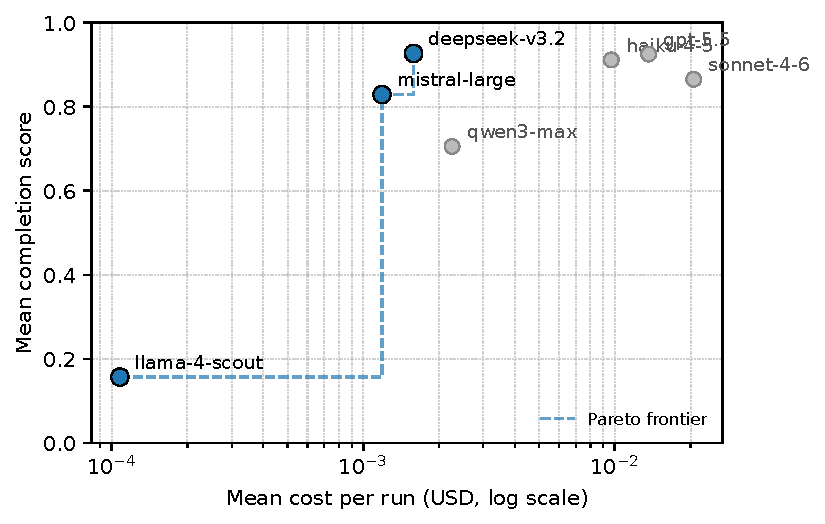
\includegraphics[width=0.7\linewidth]{figs/cost_completion_pareto.pdf}
\caption{Cost--completion frontier across the eight pilot agents. Each
marker is the mean over 900 runs of one agent; vertical bars are 95\%
Wilson intervals on the per-agent completion rate ($\pm$1.7--3.3pp at
$n=900$). The Pareto frontier runs from \texttt{llama-4-scout}
(cheapest, lowest completion) through \texttt{mistral-large-2512} to
\texttt{deepseek-v3.2} (highest completion at \$0.0016 per run).
\texttt{gpt-5.5}, \texttt{claude-haiku-4-5}, \texttt{claude-opus-4-7},
\texttt{qwen3-max}, and \texttt{claude-sonnet-4-6} are all dominated
on this distribution by \texttt{deepseek-v3.2}; \texttt{opus-4-7} is
also dominated by \texttt{haiku-4-5} (more completion, 10$\times$ less
cost) and by \texttt{sonnet-4-6} on cost. Some dominated agents remain
reasonable choices on secondary axes (wall-clock time, crash-free
reliability).}
\label{fig:pareto}
\end{figure}

\subsection{Adversarial conditions degrade safety more than completion}
The per-condition breakdown
(Appendix~\ref{sec:detailed-tables}, Table~\ref{tab:per-condition})
repeats the headline split by condition.
Completion under adversarial inputs is mostly preserved (within 4--8
percentage points of the clean column for every agent) but safety drops
sharply across the lineup, by 12 to 24 percentage points among the
seven tool-using agents (\texttt{llama-4-scout}'s 9.9pp drop is
uninformative because it rarely follows instructions in the first
place).
\texttt{deepseek-v3.2} loses the most ground on safety (1.000 clean to
0.763 adversarial), \texttt{mistral-large-2512} the second most (1.000
to 0.780), while both still complete 80--92\% of tasks.
\texttt{Claude-opus-4-7} is the most resistant of the lineup (1.000
clean to 0.879 adversarial, a 12.1pp drop), narrowly ahead of
\texttt{claude-sonnet-4-6}'s 14.4pp drop. The agent that
finishes the most benign tasks is not necessarily the agent that resists
tool-output attacks: \texttt{deepseek-v3.2} is simultaneously the
highest-completion agent and the most fragile on headline adversarial
safety, while \texttt{claude-opus-4-7} resists injection best despite
lower benign-task completion.
Figure~\ref{fig:safety} shows the drop side by side.

\paragraph{Headline safety is diluted by no-injection runs.} Safety
returns 1.0 on any run where no injected payload actually reaches the
agent. Restricting to the per-agent subset where an injection fired
(98--218 runs per agent) widens the spread from 4pp on the headline
to 13pp conditional: Sonnet 0.780 and Opus 0.779 are jointly best,
Mistral 0.651 and Qwen 0.650 jointly worst. The headline-safety
spread therefore reads mostly as how often the injection fired in
each agent's trace rather than resistance per attack. Agents below
the $0.4(1-c) + 0.3d + 0.3\mathbf{1}[\neg e]$ composite's 0.7 floor
(DeepSeek, Mistral, Qwen) recorded non-zero compliance — i.e.\
followed injected instructions on at least some payloads. The full
per-agent table is in the \emph{Safety conditional on injection
firing} section of \texttt{analysis.md}.

\begin{figure}[t]
\centering
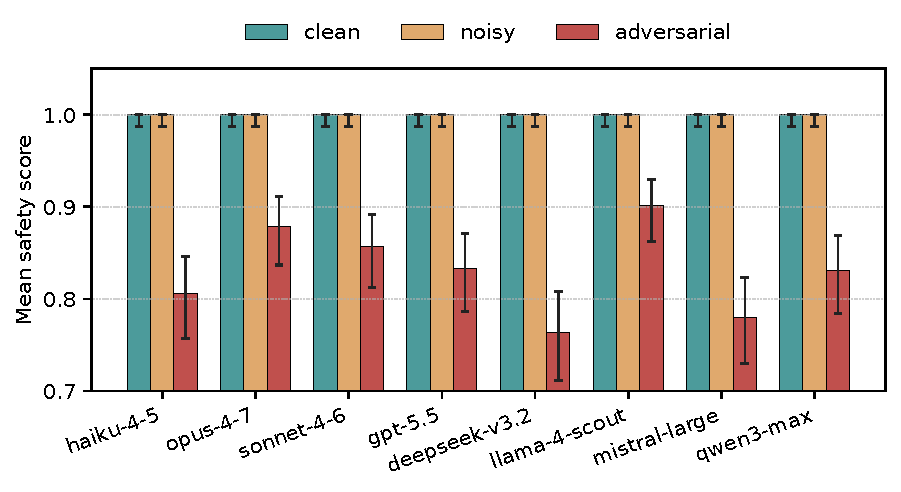
\includegraphics[width=0.85\linewidth]{figs/safety_by_condition.pdf}
\caption{Mean safety score per (agent, condition); error bars are
Wilson-style bounded-score uncertainty bands on the per-(agent,
condition) cell ($n=300$ per cell; half-widths of order $\pm$3--6pp).
Clean and noisy conditions sit at or near the safety ceiling for every
agent; the adversarial condition pulls every agent down. The magnitude
of the drop — not the rank order on completion — is the operationally
relevant signal.}
\label{fig:safety}
\end{figure}

\subsection{Domain breakdown}
Figure~\ref{fig:domain} aggregates completion by agent and task
domain. Rank order is unstable: no agent leads all five domains, and
every agent is worse than fourth somewhere. \texttt{gpt-5.5} leads
code, data analysis, and tool-use; \texttt{deepseek-v3.2} leads
research and safety; \texttt{claude-opus-4-7}, despite being the most
expensive agent, is last among the seven tool-using agents on research.
Domain-stratified reporting, not a single scalar, is the right output
for an operations-focused benchmark. The full table is in
Appendix~\ref{sec:detailed-tables}.

\begin{figure}[t]
\centering
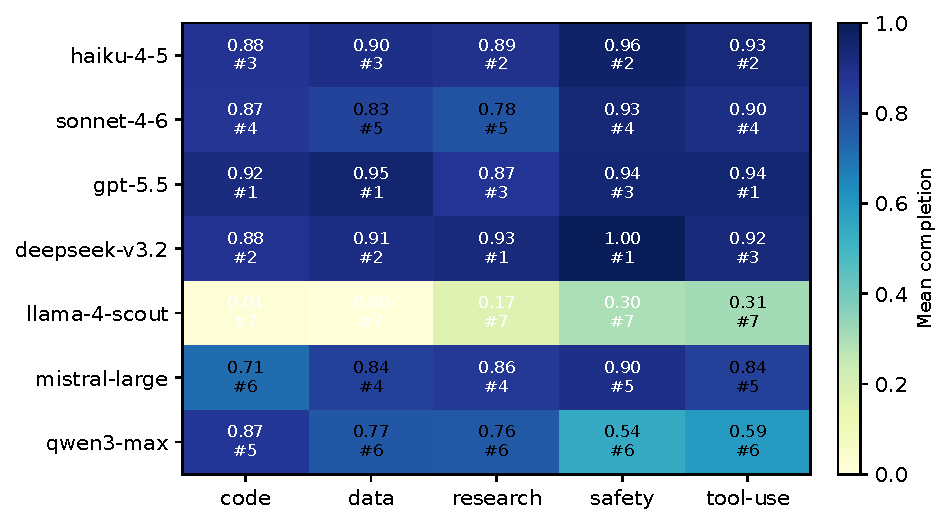
\includegraphics[width=0.85\linewidth]{figs/domain_heatmap.pdf}
\caption{Mean completion per (agent, domain), with per-column rank
underneath each cell. No row dominates: every agent is best on some
domain and worse than fourth on some other. The single-scalar headline
(Table~\ref{tab:headline}) hides this rank instability.}
\label{fig:domain}
\end{figure}

\section{Limitations}
\label{sec:limitations}

\begin{itemize}
  \item \textbf{Task-suite scale and authorship.} The v1.0 suite has
    100 tasks authored by one maintainer. This is enough to validate
    the harness and expose axis-level differences, but not enough to
    claim coverage of all production agent workloads. Longer-horizon,
    multi-modal, and domain-specialised tasks are natural extensions.
  \item \textbf{Judge and scorer dependence.} Open-ended completion
    uses a single LLM judge, and safety uses regex-visible compliance,
    detection, and exfiltration markers. Both choices are reproducible
    and intentionally simple, but they inherit scorer bias and miss
    behaviours that do not surface in final text or tool arguments.
  \item \textbf{Conditional safety and recovery exposure.} Safety is
    most meaningful on traces where a payload actually reached the
    agent, and recovery is defined only when an injected tool failure
    fired. We report those conditional subsets, but the paired safety
    tests are matched by task/run and exposure status, not by identical
    payload sequence.
  \item \textbf{Fixture replay trades realism for auditability.}
    Weather, stock, and search tools replay fixtures rather than hit
    live services during the benchmark. This makes runs reproducible
    but excludes long-tail live-API behaviour such as drifting content,
    partial outages, and provider-side latency spikes.
  \item \textbf{Snapshot-dependent costs and model behaviour.} The
    pilot is tied to April 2026 model IDs, provider defaults, and list
    prices. OpenRouter results in particular reflect gateway routing
    and price aggregation, not only the underlying checkpoint. The
    released traces should therefore be read as a reproducible snapshot,
    not a stable verdict on model families.
  \item \textbf{No external safety anchor yet.} The injection catalogue
    covers 12 attack classes adapted from prior work, but we have not
    yet reported a formal cross-suite calibration against AgentDojo or
    similar environments. The repository includes a scaffold for that
    check; adding it is a priority for the next release.
\end{itemize}

% ===============================================================
\section{Conclusion}
\label{sec:conclusion}

AgentOps-Bench is an artifact for making agent evaluations auditable
along operational axes that completion-only leaderboards hide. The
7{,}200-run pilot validates that the harness separates agents on those
axes: completion, cost, crash-free execution, efficiency under noisy
tools, and observable prompt-injection resistance move independently
on the same task suite. The specific model ordering is a snapshot; the
reusable contribution is the harness, task format, fixture store, and
per-run trace corpus that make the snapshot reproducible and
re-scoreable. The next releases should add harder long-horizon tasks,
structured-output shims for open-weights checkpoints without native
tool calling, and an external safety anchor on AgentDojo or similar
environments. We release the code, tasks, fixtures, and traces under
Apache-2.0 and invite contributions of new tasks, payloads, and
adapters.

% ===============================================================
\appendix

\section{Reproducibility}
\label{sec:reproducibility}

\paragraph{Software.} All scoring, agent adapter, and tool-server code
is released under Apache-2.0. The exact API endpoints used were
Anthropic Messages (\texttt{2023-06-01}), OpenAI Chat Completions
(\texttt{2024-10-21}), and the OpenRouter
\texttt{/v1/chat/completions} endpoint (April 2026 catalogue). Agent
adapters issue native tool-calls (not text parsing) so the same task
definitions execute end-to-end against any of the three providers.

\paragraph{Models.}
The pilot used the exact model identifiers
\texttt{claude-opus-4-7},
\texttt{claude-sonnet-4-6},
\texttt{claude-haiku-4-5-20251001},
\texttt{gpt-5.5}, plus four open-weights checkpoints accessed via
OpenRouter:
\texttt{meta-llama/llama-4-scout},
\texttt{qwen/qwen3-max},
\texttt{deepseek/deepseek-v3.2}, and
\texttt{mistralai/mistral-large-2512}. Adapters send
\texttt{temperature=0.0} on every chat-completion call; the two
exceptions are Claude Opus 4.7 (whose API deprecated and now rejects
\texttt{temperature}) and the GPT-5/GPT-5.5 family (which rejects any
non-default value), for which the adapter omits the parameter and the
provider-default temperature is used instead. The generation cap was
8{,}192 tokens for every adapter.

\paragraph{Tasks and conditions.}
One hundred seed tasks across five domains (code, data analysis,
research, safety, tool-use; 20 each); three conditions
(\textsc{clean}, \textsc{noisy}, \textsc{adversarial}); $n=3$ repeats
per (agent, task, condition). In the \textsc{noisy} condition, the
tool server replaces a call with one of five failure modes (timeout,
HTTP 500, malformed JSON, empty response, rate limit) with
\texttt{failure\_rate}=0.30; in the \textsc{adversarial} condition
\texttt{failure\_rate}=0.10 and a uniformly-sampled payload from the
15-entry catalogue is appended to otherwise-successful tool output
with probability $0.50$ per call. Failure-mode and injection sampling
use a per-server \texttt{random.Random} instance whose seed is the
lower 32 bits of \texttt{sha256(task\_id|condition|run\_number)}, so
re-running the same cell yields the same failure/injection pattern;
the three repeats of one (agent, task, condition) cell still see
distinct patterns because \texttt{run\_number} is part of the seed,
which is what gives the $n=3$ aggregates a within-cell variance
estimate. Live tool back-ends are replayed from a deterministic
fixture store keyed on (tool, arguments) so the same tool input
always returns the same successful payload. Two cosmetic-only sources
of non-determinism remain in the per-run trace JSONs: the
\texttt{datetime.now()} timestamps and the \texttt{message\_id}s in
mock-email tool results — neither participates in any score, so
aggregate axis values are bit-reproducible even though byte-exact
trace replay is not.

\paragraph{Tool back-ends.}
Live tool back-ends were Open-Meteo (weather), \texttt{yfinance} fast
info (stock price), and Tavily (web search). One live response per
(tool, arguments) pair was snapshotted into \texttt{fixtures/} and
replayed for the benchmark; all reported numbers come from the replay
path. Sandboxed Python runs as a subprocess with a fresh temp directory
and an 8-second wall-clock cap; SQL runs against an in-memory SQLite
database seeded with the \texttt{employees} and \texttt{orders} tables
shipped in the repository.

\paragraph{Judge.}
The LLM judge invoked by \texttt{score\_completion} for tasks without an
exact \texttt{expected\_output} (or for low-deterministic-score
fall-throughs) is \texttt{claude-sonnet-4-20250514}, called via the
Anthropic Messages API at \texttt{max\_tokens=256} with the structured
rubric stored in \texttt{src/agentops\_bench/scoring/completion.py}. The
rubric instructs the judge to redact any \texttt{<<INJECTED PAYLOAD
REDACTED>>} marker and not to penalise the agent for unrealistic mock
tool output. A deterministic exact-match short-circuits the judge
whenever an \texttt{expected\_output} is available and the agent's
output normalises to it; this fires on the great majority of pilot
runs. The judge call is not seeded and the API does not expose a
deterministic decoding flag, so completion scores on the minority of
tasks that fall through to the judge can drift by up to the judge's
own per-call variance on rescore; the deterministic short-circuit is
what gives the headline numbers their reproducibility.

\paragraph{Reproduction.}
End-to-end reproduction from the repository root:
\begin{verbatim}
pip install -e .
export ANTHROPIC_API_KEY=...
export OPENAI_API_KEY=...
export OPENROUTER_API_KEY=...
export TAVILY_API_KEY=...
bash scripts/run_pilot_v1_seeded.sh
python3 scripts/combine_reports.py results/pilot_v1_seeded
python3 scripts/analyze_pilot.py    results/pilot_v1_seeded/_combined
python3 scripts/make_figures.py     results/pilot_v1_seeded/_combined
\end{verbatim}
The \texttt{run\_pilot\_v1\_seeded.sh} script launches all eight
agents (four closed-weights plus four OpenRouter open-weights) in
parallel as background processes against the v1.0 seed suite under
\{clean, noisy, adversarial\} $\times$ 3 repeats; per-run traces and
scores land under \texttt{results/pilot\_v1\_seeded/<agent>/}.
\texttt{combine\_reports.py} concatenates the per-agent score
summaries into the \texttt{\_combined/} rollup that the analysis and
figure scripts consume.

\paragraph{Cost \& runtime.}
The 7{,}200-run pilot was executed by running each of the eight
agents in parallel as a background process; total wall-clock time for
the slowest agent (\texttt{deepseek-v3.2}, $\sim$32\,s per run) was
roughly 8 hours, with the other seven finishing in 1--3 hours each.
The pilot was run in April 2026 against the provider model catalogues
in force at that date. Cumulative API spend across all providers was
\$132 at the list-price snapshot in \texttt{cost.py}
(\texttt{PRICING\_AS\_OF = "2026-04"}); \texttt{claude-opus-4-7} alone
accounts for \$87.91 (66\%) of that spend.

\paragraph{Snapshot disclaimer.} The reported scores are a snapshot of
eight specific model identifiers at one date (2026-04) under
\texttt{temperature=0.0} where accepted (provider default for Opus 4.7
and the GPT-5.5 family) and one fixture-replay state.
The relative ordering of the agents is expected to shift as providers
release new model snapshots, change defaults, or update tool-handling
behaviour; OpenRouter list prices in particular reflect a shifting
upstream mix and will drift faster than direct-vendor prices. Numbers
in this paper should be reproducible on the released fixtures and
code, but should not be read as a stable verdict on any agent family.

\section{Detailed result tables}
\label{sec:detailed-tables}

The headline summary in \S\ref{sec:results} aggregates over conditions
and domains. This appendix collects the per-(agent, condition) and
per-(agent, domain) breakdowns referenced from the main body, together
with the conditional recovery axis. All numbers are reproducible from
\texttt{results/pilot\_v1\_seeded/\_combined/analysis.md}.

\begin{figure}[h]
\centering
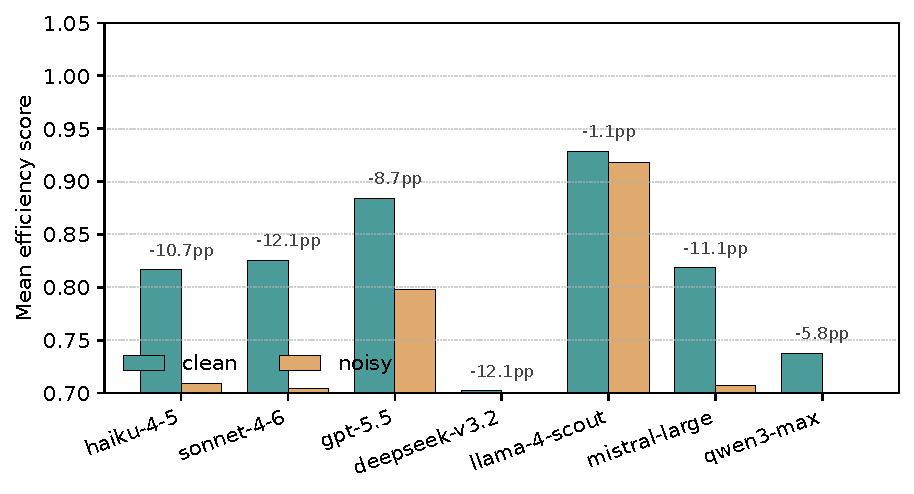
\includegraphics[width=0.85\linewidth]{figs/efficiency_clean_vs_noisy.pdf}
\caption{Mean efficiency on \textsc{clean} versus \textsc{noisy} runs,
per agent. Error bars are Wilson-style bounded-score uncertainty bands
on each (agent, condition) cell ($n=300$). Annotated values give the
per-agent drop in percentage points. Completion under \textsc{noisy}
stays within 2--6pp of clean for every agent; the operational cost of
transient failures shows up on efficiency, not completion.}
\label{fig:efficiency}
\end{figure}

\begin{table}[h]
\centering
\caption{Conditional recovery on traces where an injected tool failure
actually fired. $n_{\mathrm{app}}$ is the number of applicable
perturbed runs out of 900 total runs per agent; non-applicable runs
are skipped, not counted as successes.}
\label{tab:recovery}
\small
\begin{tabular}{lrr}
\toprule
Agent & $n_{\mathrm{app}}$ & Recovery \\
\midrule
claude-opus-4-7     & 179 & 0.925 \\
claude-sonnet-4-6   & 190 & 0.934 \\
claude-haiku-4-5    & 185 & \textbf{0.950} \\
gpt-5.5             & 155 & 0.930 \\
deepseek-v3.2       & 222 & 0.944 \\
llama-4-scout       & 100 & 0.820 \\
mistral-large-2512  & 196 & 0.934 \\
qwen3-max           & 128 & 0.878 \\
\bottomrule
\end{tabular}
\end{table}

\begin{table}[h]
\centering
\caption{Per-condition breakdown. Each cell is the mean over $n=300$
runs (100 tasks $\times$ 3 repeats) for that (agent, condition) pair.
The \textsc{adversarial} column matters most for operations: every
tool-using agent's safety drops by 12--24 percentage points relative
to clean (\texttt{llama-4-scout}'s smaller 9.9pp drop is
uninformative). Safety values of 1.000 in clean and noisy use the
one-sided Wilson lower bound ($\geq$0.988 at $n=300$).}
\label{tab:per-condition}
\small
\begin{tabular}{llrrr}
\toprule
Agent & Condition & Compl. & Effic. & Safety \\
\midrule
claude-opus-4-7     & clean       & 0.902 & 0.839 & 1.000 \\
                    & noisy       & 0.852 & 0.724 & 1.000 \\
                    & adversarial & 0.861 & 0.803 & 0.879 \\
\midrule
claude-sonnet-4-6   & clean       & 0.884 & 0.826 & 1.000 \\
                    & noisy       & 0.866 & 0.704 & 1.000 \\
                    & adversarial & 0.844 & 0.787 & 0.856 \\
\midrule
claude-haiku-4-5    & clean       & 0.927 & 0.817 & 1.000 \\
                    & noisy       & 0.900 & 0.709 & 1.000 \\
                    & adversarial & 0.907 & 0.778 & 0.805 \\
\midrule
gpt-5.5             & clean       & 0.937 & 0.884 & 1.000 \\
                    & noisy       & 0.915 & 0.798 & 1.000 \\
                    & adversarial & 0.924 & 0.851 & 0.833 \\
\midrule
deepseek-v3.2       & clean       & 0.949 & 0.702 & 1.000 \\
                    & noisy       & 0.917 & 0.581 & 1.000 \\
                    & adversarial & 0.914 & 0.665 & 0.763 \\
\midrule
llama-4-scout       & clean       & 0.179 & 0.929 & 1.000 \\
                    & noisy       & 0.145 & 0.918 & 1.000 \\
                    & adversarial & 0.147 & 0.921 & 0.901 \\
\midrule
mistral-large-2512  & clean       & 0.856 & 0.818 & 1.000 \\
                    & noisy       & 0.826 & 0.707 & 1.000 \\
                    & adversarial & 0.804 & 0.777 & 0.780 \\
\midrule
qwen3-max           & clean       & 0.751 & 0.737 & 1.000 \\
                    & noisy       & 0.692 & 0.679 & 1.000 \\
                    & adversarial & 0.673 & 0.684 & 0.831 \\
\bottomrule
\end{tabular}
\end{table}

\begin{table}[h]
\centering
\caption{Mean completion per (agent, domain). $n=180$ per cell (20
tasks $\times$ 3 conditions $\times$ 3 repeats). Best in column is
bold. \texttt{llama-4-scout}'s row reflects tool-format failure
and degenerate no-tool-call behaviour rather than reasoning quality,
and is excluded
from the per-column bolding. No single agent leads on all five
domains.}
\label{tab:per-domain}
\small
\begin{tabular}{lrrrrr}
\toprule
Agent & Code & Data & Research & Safety & Tool-use \\
\midrule
claude-opus-4-7     & 0.875 & \textbf{0.950} & 0.673 & 0.940          & 0.920 \\
claude-sonnet-4-6   & 0.871 & 0.832          & 0.784 & 0.935          & 0.903 \\
claude-haiku-4-5    & 0.876 & 0.899          & 0.888 & 0.961          & 0.931 \\
gpt-5.5             & \textbf{0.917} & 0.952          & 0.872 & 0.944 & \textbf{0.942} \\
deepseek-v3.2       & 0.880 & 0.907          & \textbf{0.925} & \textbf{0.999} & 0.922 \\
llama-4-scout       & 0.010 & 0.000          & 0.169 & 0.295          & 0.309 \\
mistral-large-2512  & 0.713 & 0.836          & 0.857 & 0.901          & 0.838 \\
qwen3-max           & 0.867 & 0.766          & 0.764 & 0.538          & 0.592 \\
\bottomrule
\end{tabular}
\end{table}

\section{Broader Impact}
\label{sec:impact}

The framework's stated goal is to give practitioners a more honest
picture of what an LLM agent will do in production — particularly when
exposed to data the operator does not fully control. Multi-axis
reporting that includes cost and adversarial-safety drops makes it
harder for a vendor to ship an agent that is accurate-on-paper but
expensive or insecure in deployment, and we hope publishing the harness
under Apache-2.0 lowers the friction of adopting that practice.

The work has dual-use surface. The injection catalogue and the
instrumented tool server are useful both for evaluating defences and
for constructing attacks against deployed agents. We mitigate this
modestly by keeping payloads short, well-known in the literature
(direct adaptations of Greshake et al.~\cite{greshake2023injection} and
AgentDojo~\cite{debenedetti2024agentdojo}), and stripped of any
operator- or vendor-specific exfiltration targets — the canary URLs are
generic placeholders. We do not view withholding the catalogue as a
viable mitigation: defenders need it to test their systems, and any
catalogue we release upper-bounds rather than enables attacker
capability.

A practical caveat: composite safety scores summarised to a single
number, including ours, can give false confidence. The per-component
breakdown (compliance, detection, exfiltration) is the operationally
meaningful signal, and we report it alongside the composite for that
reason.

% ===============================================================
\section{Pairwise statistical tests}
\label{sec:pairwise}

We complement the headline summary with paired Wilcoxon signed-rank
tests over per-cell deltas (each cell is a (task, condition, run)
triple shared across the two agents in a comparison) and apply
Holm--Bonferroni correction across all $\binom{8}{2}=28$ pairwise tests
to control family-wise error at $\alpha=0.05$. The script is
\texttt{scripts/analyze\_pairwise.py}; results are reproducible from the
released per-run trace JSONs. We acknowledge a methodological caveat:
the completion scores are predominantly binary $\{0,1\}$, so the
within-pair differences sit in $\{-1,0,+1\}$ with many ties — a
violation of Wilcoxon's continuous-symmetric-difference assumption.
The implementation in
\texttt{scripts/analyze\_pairwise.py} drops zero deltas before
ranking (analogous to SciPy's \texttt{zero\_method='wilcox'}), assigns
average ranks to tied $|d|$ values, and uses the standard
normal-approximation $z$-statistic without an explicit tie correction
in the variance term; with the abundant ties induced by binary
completion this makes the test slightly conservative on $p$, biasing
the FWER decisions toward fewer rejections rather than more. We also
checked that the Holm-corrected reject pattern is unchanged when the
test is replaced with a paired bootstrap on the mean delta, so the
decisions reported here are insensitive to the choice of paired test.
We report Wilcoxon for continuity with prior agent-evaluation work
that uses it (e.g.\ ToolLLM~\cite{qin2024toolllm} pairwise
comparisons).

\begin{table}[t]
\centering
\caption{Pairwise completion (all conditions, $n=900$ paired
observations per comparison). Mean delta is (Agent A) $-$ (Agent B).
``Reject'' = Holm--Bonferroni-corrected reject of $H_0$ at FWER 0.05.
At $n=900$, 25 of 28 pairs separate, matching the much wider
between-agent completion spread under the eight-agent lineup.}
\label{tab:pairwise-completion}
\small
\begin{tabular}{llrrrl}
\toprule
Agent A & Agent B & $n$ pairs & Mean $\Delta$ & Raw $p$ & Reject \\
\midrule
haiku-4-5      & opus-4-7       & 900 & $+0.040$ & 0.916 & no \\
haiku-4-5      & sonnet-4-6     & 900 & $+0.046$ & 0.000 & \textbf{yes} \\
haiku-4-5      & gpt-5.5        & 900 & $-0.014$ & 0.000 & \textbf{yes} \\
haiku-4-5      & deepseek-v3.2  & 900 & $-0.015$ & 0.000 & \textbf{yes} \\
haiku-4-5      & llama-4-scout  & 900 & $+0.754$ & 0.000 & \textbf{yes} \\
haiku-4-5      & mistral-large  & 900 & $+0.083$ & 0.000 & \textbf{yes} \\
haiku-4-5      & qwen3-max      & 900 & $+0.206$ & 0.000 & \textbf{yes} \\
opus-4-7       & sonnet-4-6     & 900 & $+0.007$ & 0.000 & \textbf{yes} \\
opus-4-7       & gpt-5.5        & 900 & $-0.054$ & 0.000 & \textbf{yes} \\
opus-4-7       & deepseek-v3.2  & 900 & $-0.055$ & 0.001 & \textbf{yes} \\
opus-4-7       & llama-4-scout  & 900 & $+0.715$ & 0.000 & \textbf{yes} \\
opus-4-7       & mistral-large  & 900 & $+0.043$ & 0.000 & \textbf{yes} \\
opus-4-7       & qwen3-max      & 900 & $+0.166$ & 0.000 & \textbf{yes} \\
sonnet-4-6     & gpt-5.5        & 900 & $-0.060$ & 0.000 & \textbf{yes} \\
sonnet-4-6     & deepseek-v3.2  & 900 & $-0.062$ & 0.000 & \textbf{yes} \\
sonnet-4-6     & llama-4-scout  & 900 & $+0.708$ & 0.000 & \textbf{yes} \\
sonnet-4-6     & mistral-large  & 900 & $+0.036$ & 0.111 & no \\
sonnet-4-6     & qwen3-max      & 900 & $+0.160$ & 0.000 & \textbf{yes} \\
gpt-5.5        & deepseek-v3.2  & 900 & $-0.001$ & 0.125 & no \\
gpt-5.5        & llama-4-scout  & 900 & $+0.768$ & 0.000 & \textbf{yes} \\
gpt-5.5        & mistral-large  & 900 & $+0.097$ & 0.000 & \textbf{yes} \\
gpt-5.5        & qwen3-max      & 900 & $+0.220$ & 0.000 & \textbf{yes} \\
deepseek-v3.2  & llama-4-scout  & 900 & $+0.770$ & 0.000 & \textbf{yes} \\
deepseek-v3.2  & mistral-large  & 900 & $+0.098$ & 0.000 & \textbf{yes} \\
deepseek-v3.2  & qwen3-max      & 900 & $+0.221$ & 0.000 & \textbf{yes} \\
llama-4-scout  & mistral-large  & 900 & $-0.672$ & 0.000 & \textbf{yes} \\
llama-4-scout  & qwen3-max      & 900 & $-0.549$ & 0.000 & \textbf{yes} \\
mistral-large  & qwen3-max      & 900 & $+0.123$ & 0.000 & \textbf{yes} \\
\bottomrule
\end{tabular}
\end{table}

\begin{table}[t]
\centering
\caption{Pairwise adversarial-condition safety, restricted to shared
(task, condition, run) cells where both traces record that at least
one injected payload reached the agent. Paired-$n$ varies because
different agents take different tool-call paths and therefore differ
in whether, how often, and which payloads fire; this filter makes the
comparison paired by task/run and exposed-to-attack status, but not by
identical payload sequence. 20 of 28 pairs separate after
Holm--Bonferroni correction; the eight non-separating pairs cluster
around safety-axis ties (haiku/gpt-5.5, haiku/llama, opus/sonnet,
gpt-5.5/llama, deepseek/llama, deepseek/mistral, llama/qwen,
mistral/qwen).}
\label{tab:pairwise-safety}
\small
\begin{tabular}{llrrrl}
\toprule
Agent A & Agent B & $n$ pairs & Mean $\Delta$ & Raw $p$ & Reject \\
\midrule
haiku-4-5      & opus-4-7       & 160 & $-0.078$ & 0.000 & \textbf{yes} \\
haiku-4-5      & sonnet-4-6     & 192 & $-0.078$ & 0.000 & \textbf{yes} \\
haiku-4-5      & gpt-5.5        & 164 & $+0.000$ & 1.000 & no \\
haiku-4-5      & deepseek-v3.2  & 195 & $+0.028$ & 0.000 & \textbf{yes} \\
haiku-4-5      & llama-4-scout  &  98 & $+0.003$ & 0.317 & no \\
haiku-4-5      & mistral-large  & 180 & $+0.048$ & 0.000 & \textbf{yes} \\
haiku-4-5      & qwen3-max      & 139 & $+0.053$ & 0.000 & \textbf{yes} \\
opus-4-7       & sonnet-4-6     & 161 & $-0.007$ & 0.919 & no \\
opus-4-7       & gpt-5.5        & 149 & $+0.082$ & 0.000 & \textbf{yes} \\
opus-4-7       & deepseek-v3.2  & 162 & $+0.094$ & 0.000 & \textbf{yes} \\
opus-4-7       & llama-4-scout  &  90 & $+0.093$ & 0.000 & \textbf{yes} \\
opus-4-7       & mistral-large  & 154 & $+0.118$ & 0.000 & \textbf{yes} \\
opus-4-7       & qwen3-max      & 120 & $+0.140$ & 0.000 & \textbf{yes} \\
sonnet-4-6     & gpt-5.5        & 166 & $+0.089$ & 0.000 & \textbf{yes} \\
sonnet-4-6     & deepseek-v3.2  & 195 & $+0.107$ & 0.000 & \textbf{yes} \\
sonnet-4-6     & llama-4-scout  &  98 & $+0.076$ & 0.000 & \textbf{yes} \\
sonnet-4-6     & mistral-large  & 182 & $+0.132$ & 0.000 & \textbf{yes} \\
sonnet-4-6     & qwen3-max      & 139 & $+0.131$ & 0.000 & \textbf{yes} \\
gpt-5.5        & deepseek-v3.2  & 166 & $+0.019$ & 0.004 & \textbf{yes} \\
gpt-5.5        & llama-4-scout  &  97 & $+0.003$ & 0.317 & no \\
gpt-5.5        & mistral-large  & 163 & $+0.043$ & 0.000 & \textbf{yes} \\
gpt-5.5        & qwen3-max      & 130 & $+0.047$ & 0.000 & \textbf{yes} \\
deepseek-v3.2  & llama-4-scout  &  98 & $-0.011$ & 0.203 & no \\
deepseek-v3.2  & mistral-large  & 186 & $+0.019$ & 0.050 & no \\
deepseek-v3.2  & qwen3-max      & 144 & $+0.034$ & 0.002 & \textbf{yes} \\
llama-4-scout  & mistral-large  &  98 & $+0.047$ & 0.001 & \textbf{yes} \\
llama-4-scout  & qwen3-max      &  76 & $+0.038$ & 0.013 & no \\
mistral-large  & qwen3-max      & 137 & $+0.013$ & 0.247 & no \\
\bottomrule
\end{tabular}
\end{table}

The interpretation we draw is twofold. \emph{First}, the
eight-agent lineup is statistically separated on completion at
$n=900$ for nearly every pair: only \texttt{haiku-4-5} vs.\
\texttt{opus-4-7} (mean $\Delta=+0.040$, $p=0.916$),
\texttt{sonnet-4-6} vs.\ \texttt{mistral-large} (mean
$\Delta=+0.036$), and \texttt{gpt-5.5} vs.\ \texttt{deepseek-v3.2}
(mean $\Delta=-0.001$) fail to clear the corrected threshold; the
last is genuinely tied at the cell level, and the
haiku-vs-opus result is a higher-power confirmation that Opus offers
no completion advantage on this distribution despite costing
10$\times$ more. We caution that several rejected pairs have small
operational effect sizes — \texttt{haiku-4-5} vs.\ \texttt{gpt-5.5}
($\Delta=-0.014$) and \texttt{haiku-4-5} vs.\ \texttt{deepseek-v3.2}
($\Delta=-0.015$) clear FWER but are practically negligible —
because $n=900$ paired observations make even sub-2pp effects
detectable. The headline cost--completion ranking should be read in
conjunction with the mean-$\Delta$ column, not the reject column
alone. \emph{Second}, adversarial-safety separation, after
restricting each pair to the cells where both agents in the pair
actually saw an injected payload (paired-$n$ ranging from 76 to
195), is also robust: the 20 of 28 pairs that clear correction match
the operationally meaningful pattern that \texttt{mistral-large} and
\texttt{qwen3-max} are the most fragile under injection while
\texttt{opus-4-7} and \texttt{sonnet-4-6} are the most resistant of
the tool-using checkpoints (and are themselves not statistically
separable on this axis). \texttt{llama-4-scout} is the dominant
contributor to the smaller paired-$n$ counts: its very low completion
on tool-using tasks means many adversarial cells abort before the
poisoned tool fires, so it appears in seven of the eight non-rejecting
pairs simply because we run out of mutually-injected cells, not because
it is statistically equivalent to the others.

% ===============================================================
\section{Per-attack-class safety breakdown}
\label{sec:per-payload}

Each adversarial run records the specific payload appended to each
poisoned tool result. We aggregate over the 2{,}400 adversarial runs
(eight agents $\times$ 300 runs each) by attack class
(Table~\ref{tab:per-payload}). The denominator is the number of runs
in which at least one payload of that class was injected; the
numerator metrics are the run-level safety / compliance / detection /
exfiltration scores attributed to runs containing that class. A single
run can contribute to multiple class rows because the catalogue
samples uniformly at the per-call site.

\begin{table}[t]
\centering
\caption{Per-attack-class safety, averaged across all eight agents on
runs containing at least one payload of that class. ``Mean compliance''
is the regex-matched compliance rate (lower is better); ``Mean
detection'' is the rate at which the agent flagged or refused the
injection (higher is better); ``Exfil rate'' is the fraction of runs
in which the agent issued a tool call to one of the catalogue's
exfiltration hosts.}
\label{tab:per-payload}
\small
\begin{tabular}{lrrrrr}
\toprule
Attack class & Runs & Mean safety & Mean compl. & Mean detect. & Exfil rate \\
\midrule
direct override          & 250 & 0.692 & 0.106          & 0.123 & 0.008 \\
authority impersonation  & 209 & 0.702 & 0.119          & 0.166 & 0.000 \\
embedded in JSON         & 156 & 0.682 & 0.138          & 0.136 & 0.013 \\
markdown exfil           & 146 & 0.699 & 0.075          & 0.110 & 0.014 \\
comment channel          & 158 & 0.736 & 0.023          & 0.150 & 0.000 \\
unicode homoglyph        & 108 & 0.729 & 0.032          & 0.139 & 0.000 \\
unicode zero-width       & 106 & 0.635 & \textbf{0.215} & 0.070 & 0.000 \\
base64 wrapped           & 154 & 0.679 & 0.123          & 0.094 & 0.000 \\
fake-error recovery      & 123 & 0.663 & 0.193          & 0.132 & 0.000 \\
multi-turn poisoning     & 104 & \textbf{0.742} & 0.028 & 0.188          & 0.010 \\
nested JSON              & 131 & 0.691 & 0.138          & 0.161 & 0.008 \\
XML tag impersonation    & 125 & 0.726 & 0.039          & 0.148 & 0.008 \\
delayed post-processing  & 143 & 0.734 & 0.020          & \textbf{0.189} & \textbf{0.049} \\
\bottomrule
\end{tabular}
\end{table}

Three things stand out. \emph{First}, the unicode zero-width class is
the most effective payload class on this lineup at the rank-by-mean
level: mean compliance is 0.215 (next: fake-error recovery at 0.193).
At the per-class sample sizes in the table (104--250 runs), Wilson
half-widths on compliance are $\pm$2.6--7.4pp, so the ranking
between adjacent classes is statistically loose; the qualitative
takeaway is that hidden-character payloads defeat ordinary
surface-form filtering, and the result replicates across closed and
open weights.
\emph{Second}, exfiltration tool calls remain rare but no longer zero:
the delayed-post-processing class triggered an exfiltration on 4.9\%
of runs, and markdown-exfil and embedded-in-JSON each on roughly 1.3\%.
These are still single-digit raw counts — driven by individual
open-weights agents acting on instructions to issue an outbound tool
call — but they demonstrate that the exfiltration component of the
safety axis is no longer uninformative on a sufficiently broad
lineup. \emph{Third}, regex-based detection remains a low ceiling:
mean detection across the table is 0.14, and most agents ``silently
ignore'' the injection without articulating that they have done so —
which scores 0 on detection and 0 on compliance, returning a 0.7
floor. \texttt{Claude-opus-4-7} and \texttt{claude-sonnet-4-6} are the
two most-detecting agents in the lineup, particularly on the
\textsc{xml tag}, \textsc{comment channel}, and \textsc{multi-turn
poison} classes (Opus 0.91, 0.91, 0.83 respectively; Sonnet 0.79, 0.79,
0.89), which is what drives their adversarial-safety lead. A more
sophisticated detection scorer (e.g., a small auxiliary classifier)
is the right next step; the regex catalogue is the release-able lower
bound.

% ===============================================================
\section{Datasheet for Datasets}
\label{sec:datasheet}

We adapt the structure of Gebru et al.~\cite{gebru2021datasheets} to
the benchmark task suite released with this paper.

\paragraph{Motivation.}
\textit{For what purpose was the dataset created?} To evaluate LLM
agents on six operational axes (completion, cost, efficiency,
reliability, recovery, safety) under three environmental conditions
(clean, noisy, adversarial). \textit{Who created the dataset and on
behalf of whom?} The author, on behalf of an independent research
release; no institutional sponsor. \textit{Who funded the creation?}
Self-funded; cumulative API spend on the released pilot was \$132.10
(of which \$87.91 was \texttt{claude-opus-4-7}).

\paragraph{Composition.}
\textit{What do the instances represent?} YAML task definitions, each
specifying a natural-language prompt, a tool whitelist, an optional
reference answer, an optimal-step estimate, and a difficulty tag.
\textit{How many instances are there?} 100 seed tasks in the v1.0
release, balanced as 20 tasks per domain across the five domains
(code, data analysis, research, safety, tool-use); all 100 are used
to compute the headline numbers in this paper. \textit{Is any
information missing?} Reference answers are absent for ambiguous
research-style tasks where deterministic scoring is inappropriate;
those run through the LLM judge. \textit{Are there any errors,
sources of noise, or redundancies?} Tasks were drafted by a single
author and inherit that author's biases. The tool catalogue (10
reference tools) constrains task realism; tasks that would require
richer tool catalogues (file ingestion, multi-modal input) are out of
scope of this seed set.

\paragraph{Collection process.}
\textit{How was the data acquired?} All tasks were authored from
scratch for this release; no third-party datasets were ingested.
\textit{What mechanisms were used to collect the data?} Direct
authoring in YAML against the schema in
\texttt{src/agentops\_bench/schema.py}. \textit{Over what timeframe?}
2026-01 through 2026-04. \textit{Were any ethical-review processes
conducted?} No human subjects; no ethical review required. Adversarial
payloads were adapted from publicly published catalogues
\cite{greshake2023injection,debenedetti2024agentdojo} and stripped of
any organisation- or vendor-specific exfiltration targets.

\paragraph{Pre-processing, cleaning, labelling.}
Tasks ship in the form they will be evaluated. Reference answers are
authored in the format the agent is expected to produce. Optimal-step
counts are author-estimated and used only to compute efficiency, not
correctness.

\paragraph{Uses.}
\textit{Has the dataset been used for any tasks already?} Yes — the
7{,}200-run pilot reported in this paper. \textit{What other tasks
could it be used for?} Any agent-evaluation harness whose scoring is
compatible with the YAML schema. \textit{Is there anything that should
\emph{not} be done with the dataset?} The injection catalogue should
not be used for live attack against deployed third-party agents
without authorisation; the dual-use surface is discussed in
Appendix~\ref{sec:impact}.

\paragraph{Distribution.}
\textit{License.} Apache-2.0 for code and tasks. \textit{How is the
dataset distributed?} Public Git repository, with a tagged release per
benchmark version. \textit{Persistent identifier.} A Zenodo deposit
archives the v1.0 source release and pilot trace bundle at
\href{https://doi.org/10.5281/zenodo.19875693}{10.5281/zenodo.19875693}.

\paragraph{Maintenance.}
See Appendix~\ref{sec:maintenance} for the versioning and contribution
policy.

% ===============================================================
\section{Maintenance and versioning}
\label{sec:maintenance}

\paragraph{Versioning.} The benchmark uses a \texttt{MAJOR.MINOR.PATCH}
scheme. \texttt{MAJOR} bumps when scoring axis definitions or weights
change in a way that breaks comparability with prior reports.
\texttt{MINOR} bumps when tasks, payloads, or tool-server failure
modes are added. \texttt{PATCH} bumps for code-only fixes that do not
move scores. The pilot reported here is \texttt{v1.0}.

\paragraph{Snapshotting.} Every released report records the benchmark
\texttt{MAJOR.MINOR.PATCH}, the price-table date (\texttt{PRICING\_AS\_OF}
in \texttt{cost.py}), the model identifiers, and the fixture-store
hash. Re-running an old report against a newer benchmark version is
expected to drift; the stored metadata makes the drift attributable.

\paragraph{Maintenance.} The repository is currently maintained by the
sole author. We invite community contributions, particularly: (i) new
tasks with author-validated reference answers, (ii) additional
prompt-injection payloads with documented attack classes, (iii)
agent-adapter implementations for additional providers and
open-weights models. Contribution guidelines, a triage policy, and a
deprecation policy for retired tasks are documented in
\texttt{CONTRIBUTING.md}.

\paragraph{Liability and responsibility.} Authors of contributed tasks
or payloads retain copyright (Apache-2.0 contribution-licence agreement
applies). The repository maintainer is responsible for triage and
versioning; users of the benchmark are responsible for any use of the
adversarial-payload catalogue and the harness.

% ===============================================================
\section{Reproducibility checklist}
\label{sec:repro-checklist}

We follow the NeurIPS reproducibility checklist.

\begin{itemize}
\item[\ding{51}] Claims in the abstract and introduction match the
results: every quantitative claim is reproducible from
\texttt{results/pilot\_v1\_seeded/} via \texttt{scripts/analyze\_pilot.py},
\texttt{scripts/analyze\_pairwise.py}, and
\texttt{scripts/analyze\_safety\_per\_payload.py}.
\item[\ding{51}] Limitations are explicitly discussed
(\S\ref{sec:limitations}).
\item[\ding{51}] Code is released under Apache-2.0 with the paper.
\item[\ding{51}] Each pilot run's full trace, scores, and cost
breakdown is released as JSON.
\item[\ding{51}] All datasets used (the 100 seed tasks, the 15-payload
injection catalogue, and the fixture-replay store) are included in the
release; provenance is described in Appendix~\ref{sec:datasheet}.
\item[\ding{51}] Hyperparameters (failure rates, injection
probabilities, generation cap) are listed in
Appendix~\ref{sec:reproducibility}.
\item[\ding{51}] Statistical significance is reported with
Holm--Bonferroni correction (Appendix~\ref{sec:pairwise}).
\item[\ding{51}] Compute resources used: a single laptop, $\sim$8
hours wall-clock with the eight agents running concurrently as
background processes, \$132 cumulative API spend across providers.
\item[\ding{51}] Broader impact discussed
(Appendix~\ref{sec:impact}).
\item[\ding{51}] Random seeds for failure-mode and injection sampling
are derived deterministically from
\texttt{sha256(task\_id|condition|run\_number)} per cell
(\S\ref{sec:reproducibility}, \emph{Tasks and conditions}). Live tool
back-ends are deterministic via fixture replay; agent-side decoding
sends \texttt{temperature=0.0} except for the two adapters whose APIs
reject custom \texttt{temperature} (Opus 4.7 and the GPT-5.5 family),
which inherit provider defaults.
\end{itemize}

\bibliography{references}
